\documentclass[12pt,a4paper,titlepage]{article}
\usepackage[pdftex]{graphicx}
\usepackage[polish]{babel}
\usepackage[utf8]{inputenc}
\usepackage[T1]{fontenc}
\usepackage{tabularx}
\usepackage{tikz}
\usepackage{tikz-qtree}
\usepackage{float}

\renewcommand{\labelenumii}{\arabic{enumi}.\arabic{enumii}}
\renewcommand{\labelenumiii}{\arabic{enumi}.\arabic{enumii}.\arabic{enumiii}}
\renewcommand{\labelenumiv}{\arabic{enumi}.\arabic{enumii}.\arabic{enumiii}.\arabic{enumiv}}

\tikzset{every tree node/.style={align=center,anchor=north}}

\title{Prover logiki temporalnej}
\author{Stanisław Maciąg, Piotr Mitana}
\date{2014}



\begin{document}
\newcolumntype{L}[1]{>{\raggedright\arraybackslash}p{#1}}
\newcolumntype{C}[1]{>{\centering\arraybackslash}p{#1}}
\newcolumntype{R}[1]{>{\raggedleft\arraybackslash}p{#1}}

\maketitle

\section{Założenia projektowe}
W ramach projektu zaprojektowana oraz zaimplementowana zostanie aplikacja sprawdzająca spełnialność formuły logicznej zawierającej operatory klasyczne oraz temporalne, danej w postaci ciągu znaków wprowadzonego przez użytkownika lub wczytanego z pliku. Do realizacji tego zadania wykorzystana zostanie metoda tablic semantycznych dla logiki temporalnej (ang. \textit{the Tableau Method for Temporal Logic}).

\subsection{Środowisko}
\begin{enumerate}
	\item System operacyjny Linux
	\item Języki programowania C++ oraz D
	\item Framework Qt w wersji 5
\end{enumerate}

\subsection{Implementowane funkcjonalności}
\begin{enumerate}
	\item Graficzny interfejs użytkownika (\textit{GUI}), umożliwiający wygodną obsługę aplikacji
	\item Dane wejściowe (formuły logiczne) wprowadzane ręcznie w postaci ciągu znaków, lub z pliku tekstowego (składnia wyrażeń opisana w \ref{skladnia})
	\item Wizualizacja formuły wejściowej w postaci drzewa
	\item Wizualizacja przeprowadzonego procesu dekompozycji formuły w postaci drzewa
	\item Interpretacja wynikowego drzewa dostarczająca informacji o spełnialności formuły
	\item Możliwość edycji stosowanych operatorów
\end{enumerate}

\section{Obsługa aplikacji}

\begin{figure}[H]
\centering
\includegraphics[height=12cm]{main_view}
\caption{Widok głównego okna programu}
\end{figure}

\begin{enumerate}
	\item Obszar rysowania drzewa
	\item Bieżąca formuła logiczna
	\item Przycisk otwierający okno wprowadzania formuły
	\item Przycisk definicji operatorów
	\item Informacja o wyniku działania algorytmu
	\item Przycisk inicjalizacji dekompozycji
	\item Widok na drzewo dekompozycji
	\item Widok na drzewo formuły
\end{enumerate}

\subsection{Przykład dekompozycji}

\subsubsection{Wprowadzenie formuły}
\begin{figure}[H]
\centering
\includegraphics[height=6cm]{operators_view}
\caption{Okno definicji operatorów}
\end{figure}

Program posiada możliwość edycji stosowanych operatorów logicznych i temporalnych. Powyżej przedstawiono zestaw domyślnych operatorów.

\subsubsection{Wprowadzenie formuły}
\begin{figure}[H]
\centering
\includegraphics[height=6cm]{input_view}
\caption{Okno wprowadzania formuły}
\end{figure}

Wprowadzana formuła powinna zawierać symbole operatorów zgodne ze zdefiniowanymi. Po zakończeniu edycji należy zaakceptować (1) lub odrzucić (2) zmiany. Istnieje także możliwość wczytania formuły z pliku (3). Po zdefiniowaniu formuły wejściowej użytkownikowi zostanie zaprezentowana jej wizualizacja w postaci drzewa:

\begin{figure}[H]
\centering
\includegraphics[height=6cm]{treeformula_view}
\caption{Wizualizacja formuły logicznej}
\end{figure}

\subsubsection{Dekompozycja}
\begin{figure}[H]
\centering
\includegraphics[height=6cm]{output_view}
\caption{Przedstawienie wyników}
\end{figure}

Po zakończeniu działania algorytmu program wyświetli uzyskane drzewo dekompozycji oraz informację o spełnialności formuły wejściowej. Kliknięcie na węzeł powoduje wyświetlenie jego zawartości:

\begin{figure}[H]
\centering
\includegraphics[height=6cm]{node_view}
\caption{Zawartość przykładowego węzła w drzewie dekompozycji}
\end{figure}

\section{Analiza leksykalna}

\subsection{Składnia formuły wejściowej}
\label{skladnia}
\begin{tabular}{|C{5cm}|C{5cm}|}
  \hline
  \textbf{Ciąg znaków} & \textbf{Znaczenie}\\ 
  \hline 
  Ciąg znaków alfanumerycznych & Zmienna logiczna rozumiana jako formuła atomowa\\
  \hline
  ![formuła] & Jednoargumentowy operator negacji\\
  \hline
  [formuła] \& [formuła] & Dwuargumentowy operator koniunkcji logicznej\\
  \hline
  [formuła] | [formuła] & Dwuargumentowy operator alternatywy logicznej\\
  \hline
  [formuła] \^{} [formuła] & Dwuargumentowy operator alternatywy wykluczającej\\
  \hline
  [formuła] > [formuła] & Dwuargumentowy operator implikacji logicznej\\
  \hline
  [formuła] = [formuła] & Dwuargumentowy operator ekwiwalencji logicznej\\
  \hline
  X[formuła] & Jednoargumentowy operator temporalny \textit{Next}\\
  \hline
  F[formuła] & Jednoargumentowy operator temporalny \textit{Finally}\\
  \hline
  G[formuła] & Jednoargumentowy operator temporalny \textit{Globally}\\
  \hline
  [formuła] U [formuła] & Dwuargumentowy operator temporalny \textit{Until}\\
  \hline
  ([formuła]) & Nawiasy okrągłe - grupowanie wyrażeń\\
  \hline
\end{tabular}

\subsection{Hierarchia operatorów}
\begin{tabular}{|C{5cm}|C{5cm}|}
  \hline
  \textbf{Operator} & \textbf{Priorytet}\\
  \hline
  Negacja, jednoargumentowe operatory temporalne & Najwyższy\\
  \hline
  Dwuargumentowy operator temporalny \textit{Until} & Wysoki\\ 
  \hline
  Koniunkcja, alternatywa, alternatywa wykluczająca & Średni\\
  \hline
  Implikacja, Ekwiwalencja & Najniższy\\
  \hline
\end{tabular}

\section{Algorytm działania}

\begin{figure}[!htb]
\centering
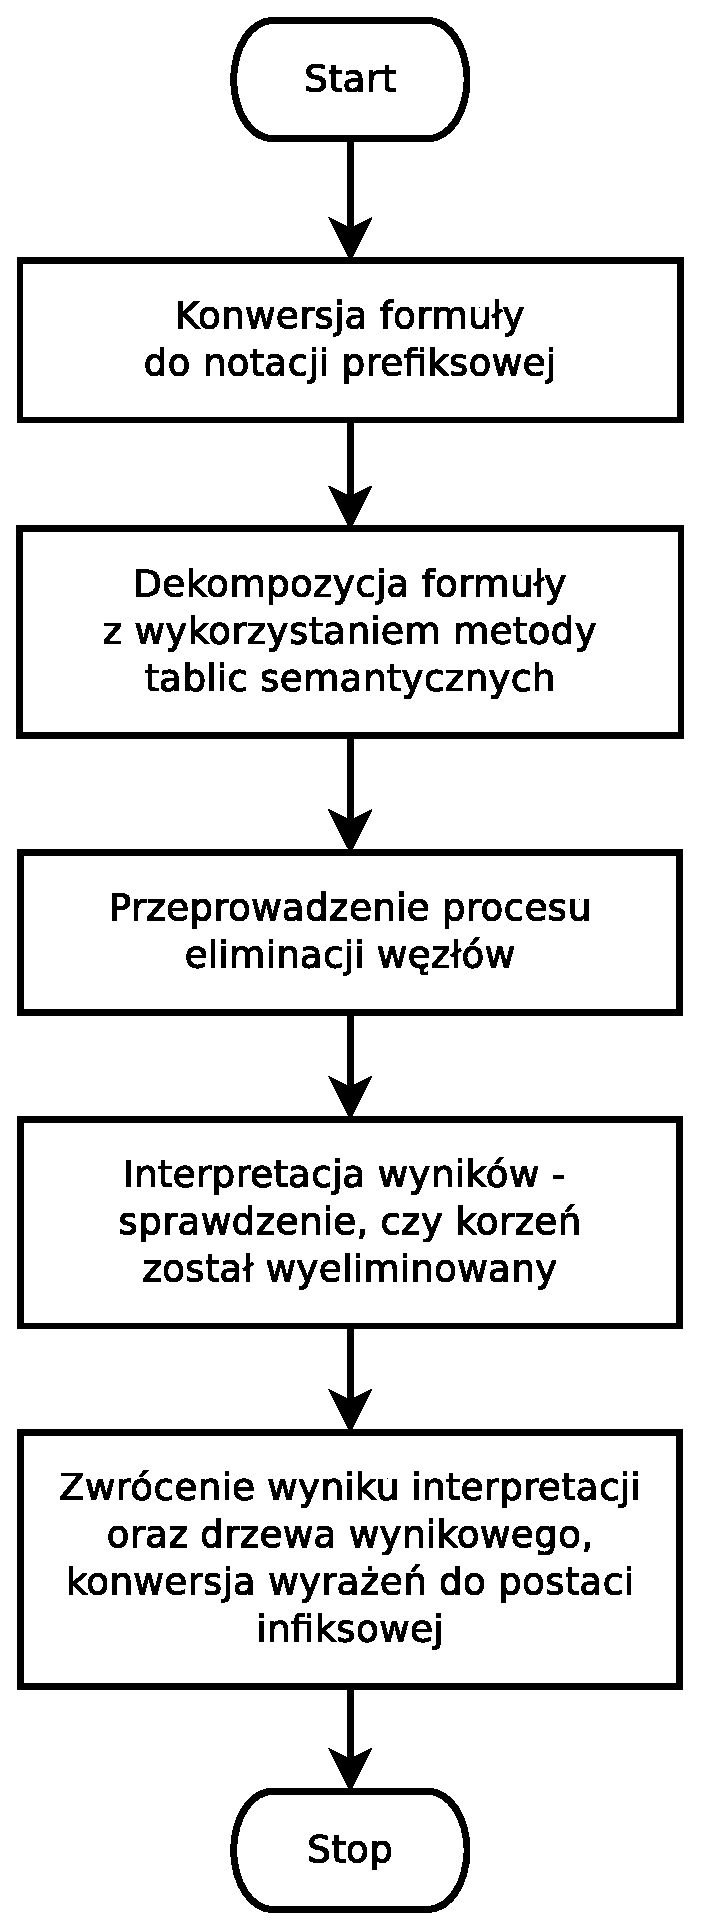
\includegraphics[height=9cm]{main_alg}
\caption{Przebieg głównego algorytmu}
\end{figure}

\subsection{Dekompozycja formuły}

\subsubsection{Reguły dekompozycji}
\label{dekompozycja}

\begin{tabular}{|C{5cm}|C{5cm}|}
\hline
\textbf{Postać dekompozycji} & \textbf{Nazwa}\\
\hline
\Tree [.{$p \wedge q$} [.{$p$ \\ $q$} ] ] &  Koniunkcja\\
\hline
\Tree[.{$p \vee q$} {$p$} {$q$} ] &  Alternatywa\\
\hline
\Tree[.{$p \Rightarrow q$} {$\neg p$} {$q$} ] &  Implikacja\\
\hline
\Tree[.{$p \Leftrightarrow q$} {$p$ \\ $q$} {$\neg p$ \\ $\neg q$} ] &  Ekwiwalencja\\
\hline
\Tree [.{$\neg(p \wedge q)$} {$\neg p$} {$\neg q$} ] &  Negacja koniunkcji\\
\hline
\Tree [.{$\neg(p \vee q)$} [.{$\neg p$ \\ $\neg q$} ] ] &  Negacja alternatywy\\
\hline
\Tree [.{$\neg(p \Rightarrow q)$} [.{$p$ \\ $\neg q$} ] ] &  Negacja implikacji\\
\hline
\Tree[.{$\neg(p \Leftrightarrow q)$} {$p$ \\ $\neg q$} {$\neg p$ \\ $q$} ] &  Negacja ekwiwalencji\\
\hline
\Tree [.{$\neg \neg p$} [.{$p$} ] ] &  Negacja negacji\\
\hline
\end{tabular}

\begin{tabular}{|C{5cm}|C{5cm}|}
\hline
\Tree [.{$\neg X p$} [.{$X \neg P$} ] ] &  Negacja operatora \textit{Next}\\
\hline
\Tree[.{$F p$} {$p$} {$X F p$} ] &  Operator \textit{Finally}\\
\hline
\Tree[.{$\neg F p$} [.{$\neg p$ \\ $\neg X F p$} ] ] & Negacja operatora \textit{Finally}\\
\hline
\Tree[.{$p U q$} {$q$} [.{$p$ \\ $X ( p U q)$} ] ] &  Operator \textit{Until}\\
\hline
\Tree [.{$\neg (p U q) $} [.{$\neg q$ \\ $\neg p \vee \neg X (p U q)$} ] ] &  Negacja operatora \textit{Until}\\
\hline
\Tree[.{$G p$} {$p$} {$X G p$} ] &  Operator \textit{Globally}\\
\hline
\end{tabular}

\subsubsection{Algorytm metody tablic semantycznych}
\begin{enumerate}
	\item Tworzenie korzenia drzewa zawierającego formułę wejściową (lub jej zaprzeczenie)
	\item Dekompozycja następnego w kolejności wyrażenia logicznego. Kolejność dekomponowania wyrażeń znajdujących się w węzłach drzewa jest dowolna, jednak ze względu efektywność algorytmu najlepiej przyjąć następujący porządek:
	\begin{itemize}
	\item[1] Dekomponowanie wyrażeń niepowodujących rozgałęziania
	\item[2] Dekomponowanie wyrażeń powodujących rozgałęzianie oraz tworzących dwa pod-wyrażenia w węzłach potomnych
	\item[3] Dekomponowanie wyrażeń powodujących rozgałęzianie oraz tworzących jedno wyrażenie w węzłach potomnych
	\end{itemize}
	\item W przypadku węzła, który zawiera wyrażenia z operatorem \textit{Next} - rozszerzenie drzewa, przez przyłączenie potomka zawierającego wyrażenia nieatomiczne, z usuniętym zewnętrznym operatorem \textit{Next}, lub w przypadku gdy takie wyrażenie już występowało w nadrzędnym węźle, utworzenie ścieżki do tego węzła
	\item Dekompozycję powtarza się, w każdym węźle nie zostaną sprawdzone wszystkie wyrażenia
	\item Eliminacja węzłów - węzeł oznacza się jako usunięty, jeśli:
	\begin{itemize}
	\item[1] Zawiera on dwie osobne formuły, które są zmienną logiczną i jej zaprzeczeniem
	\item[2] Wszyscy potomkowie węzła zostali usunięci
	\item[3] Jeśli węzeł zawiera operatory temporalne $F p$ lub $q U p$ i jeśli nie istnieje w drzewie ścieżka prowadząca do węzła zawierającego formułę $p$ 
	\end{itemize}
	\item Interpretacja wyników - jeżeli korzeń drzewa został usunięty, to formuła jest niespełnialna (w przypadku, gdy w korzeniu zostało podane jej zaprzeczenie jest spełnialna)
\end{enumerate}

\end{document}